\section{Theorie}
\label{sec:Theorie}

\subsection{Begriffe aus der Elastizitätstheorie}
\label{sec:begriffe}

\subsubsection{Volumen- und Oberflächenkräfte}
Kräfte, die an Festkörpern angreifen, lassen sich in Volumenkräfte und Oberflächenkräfte
unterteilen. Letztere werden in diesem Versuch genauer betrachtet.
Volumenkräfte wirken auf jedes Volumenelement des Festkörpers und können Translationsbewegungen
und Rotationsbewegungen hervorrufen.
Im Gegensatz dazu können \textbf{Oberflächenkräfte} -- Kräfte, die an Oberflächenelementen
angreifen -- Gestalts- und Volumenänderungen bewirken. Sie können neben der Oberfläche auch an
jeder Querschnittsfläche des Körpers nachgewiesen werden.

\subsubsection{Die Spannung}
Es wird der Begriff der \textbf{Spannung} eingeführt, welche als Oberflächenkraft pro Fläche
definiert ist. Des Weiteren unterscheidet man zwischen der \textbf{Normalspannung $\sigma$}
(auch \textbf{Druck $P$}) und der \textbf{Tangentialspannung $\tau$} (auch
\textbf{Schubspannung}), welche dem orthogonalen bzw. dem tangentialen Anteil der Spannung
entsprechen.

Wirkt eine Spannung auf einen Festkörper, treten Verformungen -- in Form von Gestalts- und
Volumenänderungen -- auf. Diese Verformungen entsprechen auf molekularer Ebene einem veränderten
Gleichgewichtszustand der Atom- bzw. Molekülstruktur, der durch die elektrostatischen
Kräfte zwischen den Atomen bzw. Molekülen eintritt. Wenn die wirkende Spannung abgenommen wird
und der Körper in seinen ursprünglichen Zustand -- mit gleicher Form und Größe -- zurückkehrt,
spricht man von einer \textbf{elastischen Deformation}.

\subsubsection{Elastizitätskonstanten}
Weiterhin ergibt sich ein proportionaler Zusammenhang zwischen der Deformation -- in Form
einer relativen Längen- oder Volumenänderung $\frac{\Delta L}{L}$ bzw.
$\frac{\Delta V}{V}$ -- und der Spannung, wenn der Betrag der wirkenden Oberflächenkraft nicht
zu groß ist, was in Abbildung \ref{fig:Hooki} durch den Hookeschen Bereich illustriert ist.
\begin{figure}
	\centering
	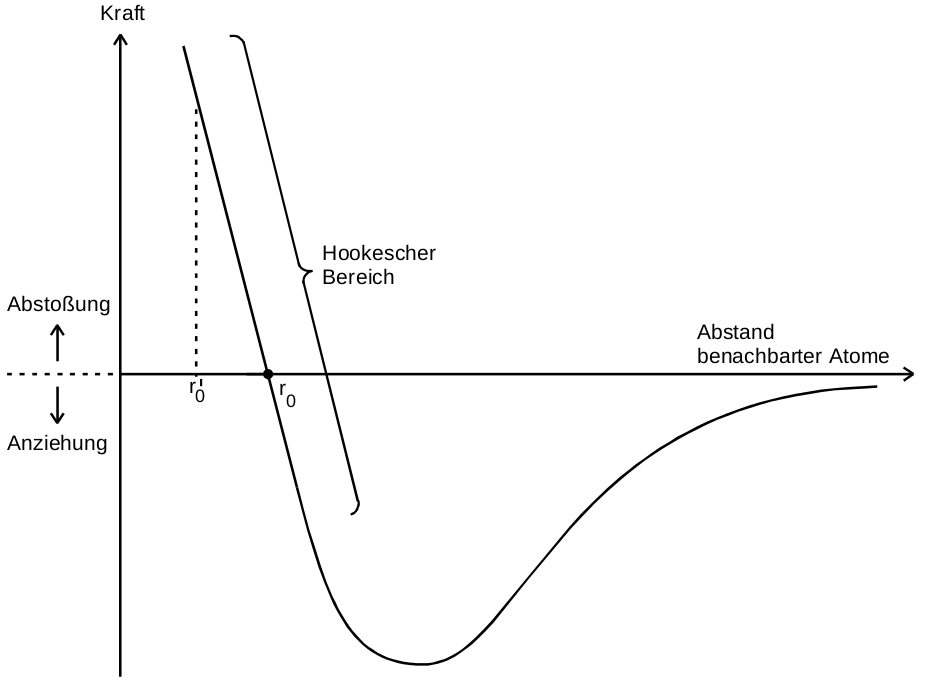
\includegraphics[width=0.75\textwidth]{Bilder/HookscherBereich.png}
	\caption{Schematischer Verlauf der Kraft zwischen benachbarten Atomen ($r_{\mathrm{0}}$=Gleichgewichtsabstand).  \cite{Anleitung}}
	\label{fig:Hooki}
\end{figure}
Liegt die Kraft in diesem Bereich, wird ein proportionaler Zusammenhang angenommen, der sich zu
\begin{align}
	\label{eqn:elastimodi}
	  & \sigma = E \, \frac{\Delta L}{L} \,\,\,\, \mathrm{oder} & P = Q \, \frac{\Delta V}{V}
\end{align}
ergibt.

Allgemein werden 36 Konstanten (jeweils 6 Konstanten zur Charakterisierung der Spannung und
Deformation) in Form einer Matrix benötigt, um den proportionalen Zusammenhang zwischen
Spannung und Deformation zu beschreiben.
Zusätzlich ist das Schema der Elastizitätskonstantenmatrix symmetrisch \cite{Ergebnis der
exakten Naturwissenschaften vierter band , googlen 21 elastsoooss}, sodass im allgemeinen Fall
21 Elastizitätskonstanten benötigt werden.
Im sogenannten kubischen Kristallsystem verbleiben aufgrund weiterer Symmetrien 3 notwendige
Elastizitätskonstanten und bei \textbf{isotropen Körpern} -- Körper mit richtungsunabhängigen
Elastizitätskonstanten -- wird diese Anzahl auf nur 2 reduziert.

Diese 2 Konstanten werden als \textbf{Schubmodul $G$} (auch \textbf{Torsionsmodul}) und
\textbf{Kompressionsmodul $Q$} bezeichnet.
Letztere ist eine Kenngröße für die Volumenelastizität. Der Schubmodul charakterisiert die
Gestaltselastizität.

Weiterhin definiert man in der Praxis zwei weitere Konstanten: der
\textbf{Elastizitätsmodul $E$} und die \textbf{Poissonsche Querkontraktionszahl $\mu$}.

Der Elastizitätsmodul wurde in Gleichung \eqref{eqn:elastimodi} definiert und ist der
Proportionalitätsfaktor zwischen dem Druck $P$ und der relativen Volumenänderung
$\frac{\Delta V}{V}$.
Bewirkt eine Oberflächenspannung $\vec{\sigma}$ an einem Festkörper eine Längenänderung,
entspricht die Poissonsche Querkontraktionszahl $\mu$ dem Proportionalitätsfaktor zwischen
der Längenänderung parallel zur Spannungsrichtung $\frac{\Delta L}{L}$ und der Längenänderung
orthogonal zur Spannungsrichtung $\frac{\Delta B}{B}$. Die Poissonsche Querkontraktionszahl
wird in Abbildung \ref{fig:querkontrakti} durch das Beispiel eines gedehnten Stabes erklärt und
als
\begin{equation*}
	\mu := - \frac{\Delta B}{B} \cdot \frac{L}{\Delta L}
\end{equation*}
\begin{figure}
	\centering
	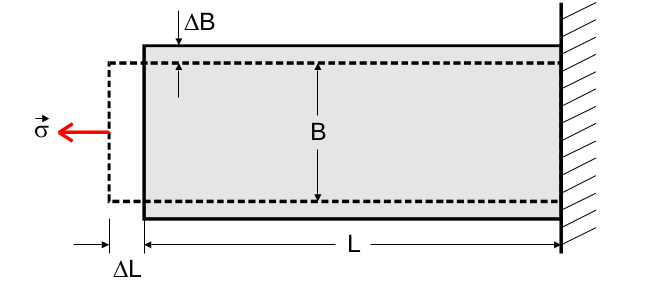
\includegraphics[width=0.7\textwidth]{Bilder/Querkontraktion.png}
	\caption{Poissonsche Querkontraktionszahl $\mu$ erklärt an einem gedehnten Stab. \cite{Anleitung}}
	\label{fig:querkontrakti}
\end{figure}
definiert.

Da bei isotropen Körpern nur zwei Konstanten benötigt werden, müssen die zwei zusätzlichen
Konstanten durch zwei Gleichungen miteinander verknüpft sein.
Diese Zusammenhänge ergeben sich zu
\begin{align}
	E & = 2G (\mu + 1) \mathrm{,}  \\
	E & = 3Q (1 - 2\mu) \mathrm{.}
\end{align}
\FloatBarrier

\subsection{Bestimmung des Schubmoduls $G$}

Der Schubmodul $G$ ist eine Kenngröße für die Gestaltselastizität eines Körpers und entspricht
dem Proportionalitätsfaktor zwischen einer Tangentialspannung $\tau$ und einem Scherungswinkel
$\alpha$:
\begin{equation}
	\label{eqn:schubimoduli}
	\tau = G \alpha \mathrm{.}
\end{equation}
Die dem Schubmodul $G$ zugehörige Deformation wird also als \textbf{Scherung} bezeichnet.
Diese Deformation ist durch eine an einem Körper angreifende Tangentialspannung bedingt, die
den Körper -- wie in Abbildung \ref{fig:würfeli} illustriert -- um einen Scherungswinkel $\alpha$
neigt.
\begin{figure}
	\centering
	\includegraphics[width=0.4\textwidth]{Bilder/Würfel_Schubspannung.png}
	\caption{Darstellung der durch die Schubspannung verursachte elastische Deformation. \cite{Anleitung}}
	\label{fig:würfeli}
\end{figure}
Da der Scherungswinkel $\alpha$ in Abbildung \ref{fig:würfeli} allerdings nur schwierig zu messen
ist, wird im Folgenden die Torsion eines Zylinders betrachtet.

\subsubsection{Die Torsion eines Zylinders}
\label{sec:torsionii}
\begin{figure}
	\centering
	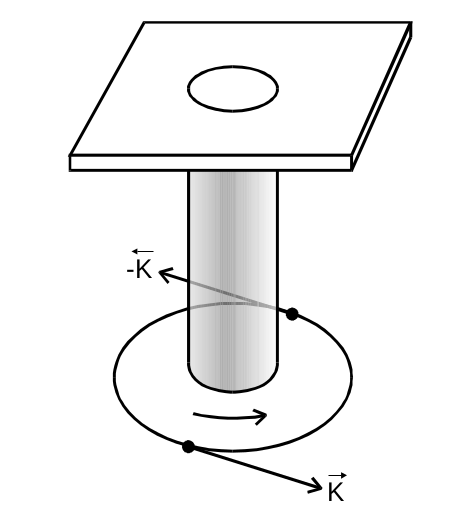
\includegraphics[width=0.4\textwidth]{Bilder/Torsion_Schubmodul.png}
	\caption{Torsion eines zylindrischen Stabes. \cite{Anleitung}}
	\label{fig:torsioni}
\end{figure}
Der Zylinder ist an einem Ende fest eingespannt und wird am anderen Ende durch zwei
gegenüberliegende, in entgegengesetzte Richtung wirkende Kräfte gedrillt (siehe Abbildung
\ref{fig:torsioni}).
Durch diese Kräfte wirkt ein Drehmoment $M$ auf den Zylinder und erzeugt eine Drehung des losen
Endes des Zylinders gegenüber dem fest eingespannten Ende des Zylinder. Diese Drehung wird
durch den Torsionswinkel $\varphi$ festgelegt.
Da das Drehmoment über den Durchmesser des Zylinders variiert, wird der Zylinder in Hohlzylinder
mit dem Radius $r$ und Dicke $\symup{d} r$ zerlegt, von denen sich die einzelnen Drehmomente
über den gesamten Zylinderradius integrieren lassen, sodass man das Gesamtdrehmoment $M$
erhält.

Des Weiteren legt der Torsionswinkel $\varphi$ den Scherungswinkel $\alpha$ zwischen den
Mantelschichten fest, wie in Abbildung \ref{fig:verdrilltorsion} dargestellt.
\begin{figure}
	\centering
	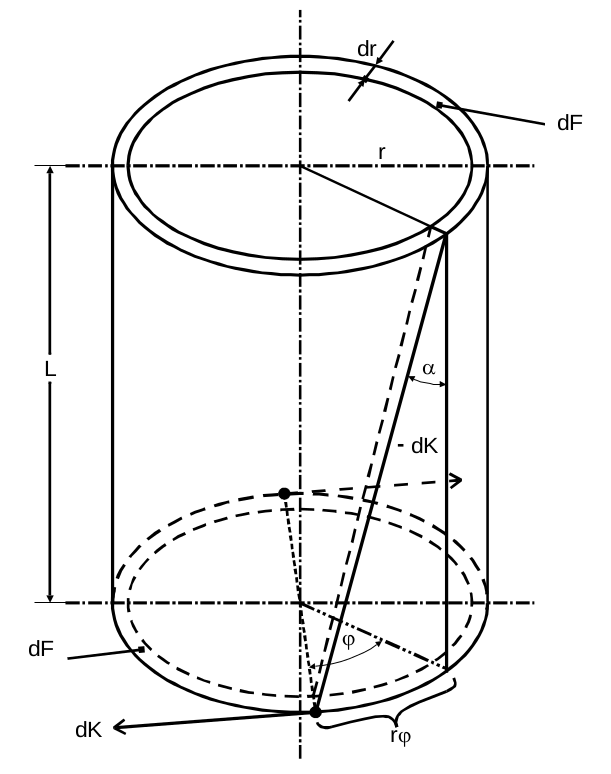
\includegraphics[width=0.5\textwidth]{Bilder/Zylinder_Verdrillung.png}
	\caption{Darstellung des Zusammenhangs zwischen Drehmoment $M$ und Verdrillungswinkel $\phi$. \cite{Anleitung}}
	\label{fig:verdrilltorsion}
\end{figure}
Es ergibt sich der Zusammenhang zwischen Torsionswinkel $\varphi$ und Scherungswinkel $\alpha$
zu
\begin{equation}
	\label{eqn:variphi}
	\alpha = \frac{r \varphi}{L} \mathrm{,}
\end{equation}
mit der Länge $L$ und dem Radius $r$ der Hohlzylinder.

Mit Gleichung \eqref{eqn:schubimoduli} soll nun ein Zusammenhang zwischen dem Drehmoment $M$
und dem Torsionswinkel $\varphi$ gefunden werden.
Das infinitiesimale Drehmoment $\symup{d} M$, welches auf einen Punkt mit der Entfernung $r$
zur Zylinderachse wirkt, ergibt sich durch
\begin{equation*}
	\symup{d} M = r \, \symup{d}K \mathrm{,}
\end{equation*}
wobei $\symup{d} K$ der Tangentialkraft entspricht.
Weiterhin ist die Tangentialspannung $\tau$ aus Gleichung \eqref{eqn:elastimodi} als
Tangentialkraft pro Flächeneinheit
\begin{equation*}
	\tau = \frac{\symup{d} K}{\symup{d} F}
\end{equation*}
definiert.
Mit diesen beiden Definitionen und Gleichungen \eqref{eqn:schubimoduli} und \eqref{eqn:variphi}
ergibt sich das Drehmoment eines Hohlzylinders $\symup{d} M$ zu
\begin{equation}
	\symup{d} M = 2\pi \frac{G}{L} \varphi r^3 \symup{d}r \mathrm{.}
\end{equation}
Integration über den Zylinderradius $R$ liefert das Drehmoment
\begin{equation}
	\label{eqn:drehmoment}
	M = \int_0^R \symup{d} M = \frac{\pi}{2} G \frac{R^4}{L} \varphi \mathrm{.}
\end{equation}
Die Gleichung \eqref{eqn:drehmoment} entspricht also einem abgewandelten Hookeschen Gesetz
mit dem Proportionalitätsfaktor
\begin{equation}
	\label{eqn:richti}
	D := \frac{\pi G R^4}{2L} \mathrm{,}
\end{equation}
der als Richtgröße des Zylinders bezeichnet wird.

Gleichung \eqref{eqn:drehmoment} ermöglicht es theoretisch -- nach der Messung der unbekannten
Größen -- den Schubmodul $G$ zu bestimmen.
Diese Methode wird allerdings in der Praxis nicht verwendet, da durch die \textbf{elastischen
Nachwirkung} eine mögliche Fehlerquelle entstehen kann.
Die elastische Nachwirkung beschreibt das Phänomen, dass einige Stoffe nach dem Aufgeben der
Spannung nicht sofort wieder in den Ausgangszustand zurückkehren.

Daher wird in der Praxis die sogenannte dynamische Methode verwendet, bei der die Spannung
einer periodischen Funktion der Zeit entspricht.

\subsubsection{Die dynamische Methode}
\label{sec:dynamisch}
Bei der dynamischen Methode wird das Beispiel aus Abschnitt \ref{sec:torsionii} mit einem Körper
mit Trägheitsmoment $\theta$ am freien Ende des Zylinders erweitert.
Das Drehmoment $M_{\mathrm{T}}$  des Körpers ergibt sich zu
\begin{equation}
	M_{\mathrm{T}} = \theta \frac{\symup{d}^2 \varphi}{\symup{d} t^2} \mathrm{.}
\end{equation}
Wird nun der Zylinder ausgelenkt, wirken zwei entgegengesetzte Drehmomente: Das Drehmoment
durch die Torsion des Zylinders und das Drehmoment bedingt durch die Trägheit des Körpers.

Dadurch entsteht eine Drehschwingung mit der Differentialgleichung
\begin{equation}
	D \varphi + \theta \frac{\symup{d}^2 \varphi}{\symup{d} t^2} \mathrm{.}
\end{equation}
Die Lösung der Differentialgleichung ergibt sich durch
\begin{equation}
	\varphi(t) = \varphi_0 \cos(\frac{2\pi}{T} t) \mathrm{,}
\end{equation}
wobei
\begin{equation}
	\label{eqn:toughtimes}
	T = 2\pi \sqrt{\frac{\theta}{D}}
\end{equation}
der Schwingungsdauer der ungedämpften Schwingung -- unter Vernachlässigung von
Reibungskräften -- entspricht.

\subsubsection{Bestimmung des Trägheitsmomentes}

Das Trägheitsmoment $\theta$ ist als
\begin{equation*}
	\theta = \int_V \, \vec{r}_{\perp} \, \rho(\vec{r}) \symup{d} V
\end{equation*}
definiert, mit dem Vektor $\vec{r}_{\perp}$, der den Abstand eines Massenelementes zur
Roatationsachse festlegt.

Im Versuch wird eine Kugel mit homogener Masseverteilung verwendet.
Das Trägheitsmoment $\theta_{mathrm{Kugel}}$ ergibt sich zu
\begin{equation*}
	\theta_{\mathrm{Kugel}} = \frac{8}{15} \pi \rho R_{\mathrm{k}}^5 \mathrm{,}
\end{equation*}
mit dem Kugelradius $R_{\mathrm{k}}$.
Mit der Kugelmasse
\begin{equation*}
	m_{\mathrm{k}} = \frac{4}{3} \pi R_{\mathrm{k}}^3 \rho
\end{equation*}
ergibt sich das Trägheitsmoment einer Kugel schließlich zu
\begin{equation}
	\label{eqn:trägee}
	\frac{2}{5} m_{\mathrm{k}} R_{\mathrm{k}}^2 \mathrm{.}
\end{equation}

Aus den Gleichungen \eqref{eqn:richti}, \eqref{eqn:toughtimes} und \eqref{eqn:trägee} ergibt
sich schließlich der Schubmodul $G$ zu
\begin{equation}
	\label{eqn:schubischu}
	G = \frac{16}{5} \pi \frac{m_{\mathrm{k}} R_{\mathrm{k}}^2 L}{T^2 R^4} \mathrm{.}
\end{equation}


\FloatBarrier
\subsection{Das magnetische Moment eines Permanentmagneten}

Das magnetische Moment $\vec{m}$ ist als
\begin{equation}
	\vec{m} := p \vec{a}
\end{equation}
definiert, wobei $p$ der Polstärke und $\vec{a}$ einem Vektor vom Nordpol zum Südpol mit dem
Betrag vom Abstand der beiden Pole entspricht.
\begin{figure}
	\centering
	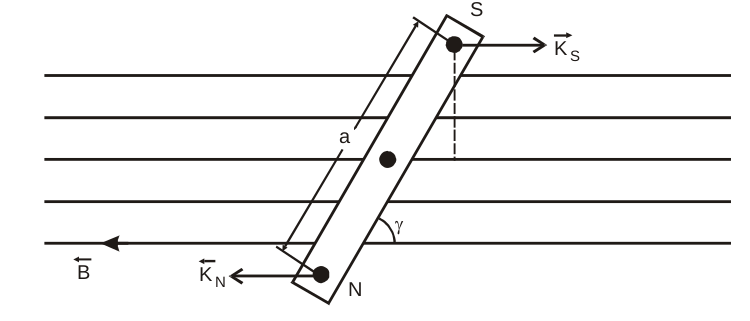
\includegraphics[width=0.7\textwidth]{Bilder/Magnet.png}
	\caption{Angreifende Kräfte an einem stabförmigen Permanentmagneten in einem äußeren Magnetfeld. \cite{Anleitung}}
	\label{fig:magnetus}
\end{figure}

Befindet sich dieser Magnet in einem homogenen, äußeren Magnetfeld $\vec{B}$, wirken zwei
Kräfte an dem Magnetenm, die am Nordpol und Südpol angreifen (siehe Abbildung \ref{fig:magnetus}.
Da diese Kräfte den gleichen Betrag haben, führt der Magnet keine Translationsbewegung aus
sondern rotiert durch das Drehmoment $M_{\mathrm{Mag}}$ in Feldrichtung.
Das Drehmoment $M_{\mathrm{Mag}}$ ergibt sich zu
\begin{equation}
	M_{\mathrm{Mag}} = p \vec{a} \times \vec{B} = \vec{m} \times \vec{B} \mathrm{.}
\end{equation}
Das magnetische Moment $\vec{m}$ kann mit der dynamischen Methode aus Abschnitt
\ref{sec:dynamisch} bestimmt werden, indem zusätzlich der Permanentmagnet in die Kugel eingebaut
wird und ein homogenes Magnetfeld erzeugt.
Die abgeänderte Anordnung ergibt wieder periodische Schwingungen, allerdings mit einer
abweichenden Periodendauer $T_{\mathrm{m}} \neq T$.

Richtet man den Magneten parallel zur Feldrichtung aus entspricht $\gamma$ aus Abbildung
\ref{fig:magnetus} dem Torsionswinkel $\varphi$ und es ergibt sich die Differentialgleichung
\begin{equation}
	m B \sin(\varphi)  + D \varphi + \theta \frac{\symup{d}^2 \varphi}{\symup{d} t^2} = 0
	\mathrm{.}
\end{equation}
Diese nicht-lineare Differentialgleichung lässt sich mit einer Kleine-Winkel-Näherung
\begin{equation*}
	\sin(\varphi) \approx \varphi + \symup{o}(\varphi^2)
\end{equation*}
schreiben als
\begin{equation}
	(mB + D) \varphi + \theta \frac{\symup{d}^2 \varphi}{\symup{d} t^2} = 0 \mathrm{.}
\end{equation}
Die Lösung dieser linearen Differentialgleichung hat die Form
\begin{equation}
	\varphi(t) = \varphi_0 \cos(\frac{2\pi}{T_{\mathrm{m}}} t \mathrm{,}
\end{equation}
mit der neuen Periodendauer
\begin{equation}
	T_{\mathrm{m}} = 2\pi \sqrt{\frac{\theta}{mB + D}} \mathrm{.}
\end{equation}
